% !TEX root = master.tex
\chapter{Einführung} \label{chapter:1}
%Darstellung des Problems, der Umgebung mit Regeln/ Dynamik und ggf. Vereinfachungen.

Im Rahmen dieser Gruppenarbeit mit dem Ziel der Implementierung von erlernten \acf{RL} Verfahren wurde sich für das ``Soccer Twos''-Problem \cite[p. 15]{juliani2020} entschieden. Es handelt sich hierbei um eine, als Teil des ``Unity \ac{ML} Agents Toolkit'' \cite{juliani2020} veröffentlichte, Umgebung, welche ein vereinfachtes Fußballspiel zwischen zwei Teams mit je zwei Spielern simuliert und somit ein \acf{MARL} Problem darstellt.
Die Entscheidung für dieses \ac{RL}-Problem wurde getroffen, auf Grundlage der geigneten Anwendungsmöglichtkeit von den in der Veranstaltung behandelten Verfahren, sowie den Anspruch auf eine durchaus herausfordernde Aufgabe, welche durch die erhöhte Komplexität des Multi-Agent Problem hier gegeben ist. 

\section{Soccer Twos Umgebung}

Das Unity \ac{ML} Agents Toolkit verfügt über diverse Komponenten um \ac{RL} verwandte Aspekte in Unity-Umgebungen umzusetzen und bietet zudem eine Vielzahl an Beispiel-Umgebungen und Implementierungen von \ac{RL}-Algorithmen, welche es Spieleentwicklern oder Forschern ermöglicht \ac{RL}-Verfahren zu entwicklen und testen. 
Die bereitgestellten Beispielumgebungen zeigen die Einsatzmöglichkeiten des Toolkits durch kleinere Spiele, die größtenteils in einer 3D-Umgebung stattfinden, auf. In den Umgebungen agieren einfache blockförmige und auch komplexere mit Gelenken ausgestattete Agenten, die alleine oder gemeinsam verschiedene Aufgaben lösen müssen. Die Beobachtungsräume dieser Agent sind größtenteils in Vektorform dargestellt sowie in einzellnen Fällen auch visuell und die Aktionsräume sind je nach Spiel entweder diskret oder kontinuierlich. Dies bietet somit eine Ausgangslage für die Anwedung von \ac{RL}-Verfahren in unterschiedlichstem Umfang.

Da das Toolkit mit seinem beträchtlichen Funktionsumfang bereits eine gewisse Komplexität aufweist, wurde entschieden, das Projekt in einer ausschließlich Python-basierten Gymnasium-Umgebung umzusetzen und dementsprechend ein passendes Paket zu nutzen \cite{soccertwos}. Dieses Paket ermöglichte es, die komplette Implementierung in Python durchzuführen und die bereits bekannten Gymnasium-Schnittstellen zu nutzen.

Beim Spiel ``Soccer Twos'' spielen zwei Agenten gemeinsam in einem Team gegen ein weiteres Zweier-Team Fußball. Es handelt sich hierbei um eine 3D-Spielumgebung, die in Abbildung \ref{fig:soccer_twos_3d} dargestellt ist. Das Spielfeld ist mit einer Bande begrenzt, wodurch es kein Aus gibt und das Spiel nicht unterborchen wird. Zu Beginn eines Spiels liegt der Ball in der Mitte des Feldes, und die beiden Teams starten auf ihrer jeweiligen Seite des Spielfelds. Die Agenten sind nicht unbedingt in der Lage, komplexe bzw. sehr präzise Schüsse auszuführen, sondern passen und schießen lediglich, indem sie einfach gegen den Ball laufen. Es ist das Ziel jedes Teams, den Ball in das gegnerische Tor zu befördern und gleichzeitig das eigene Tor zu schützen.

\begin{figure}[h]
	\centering
	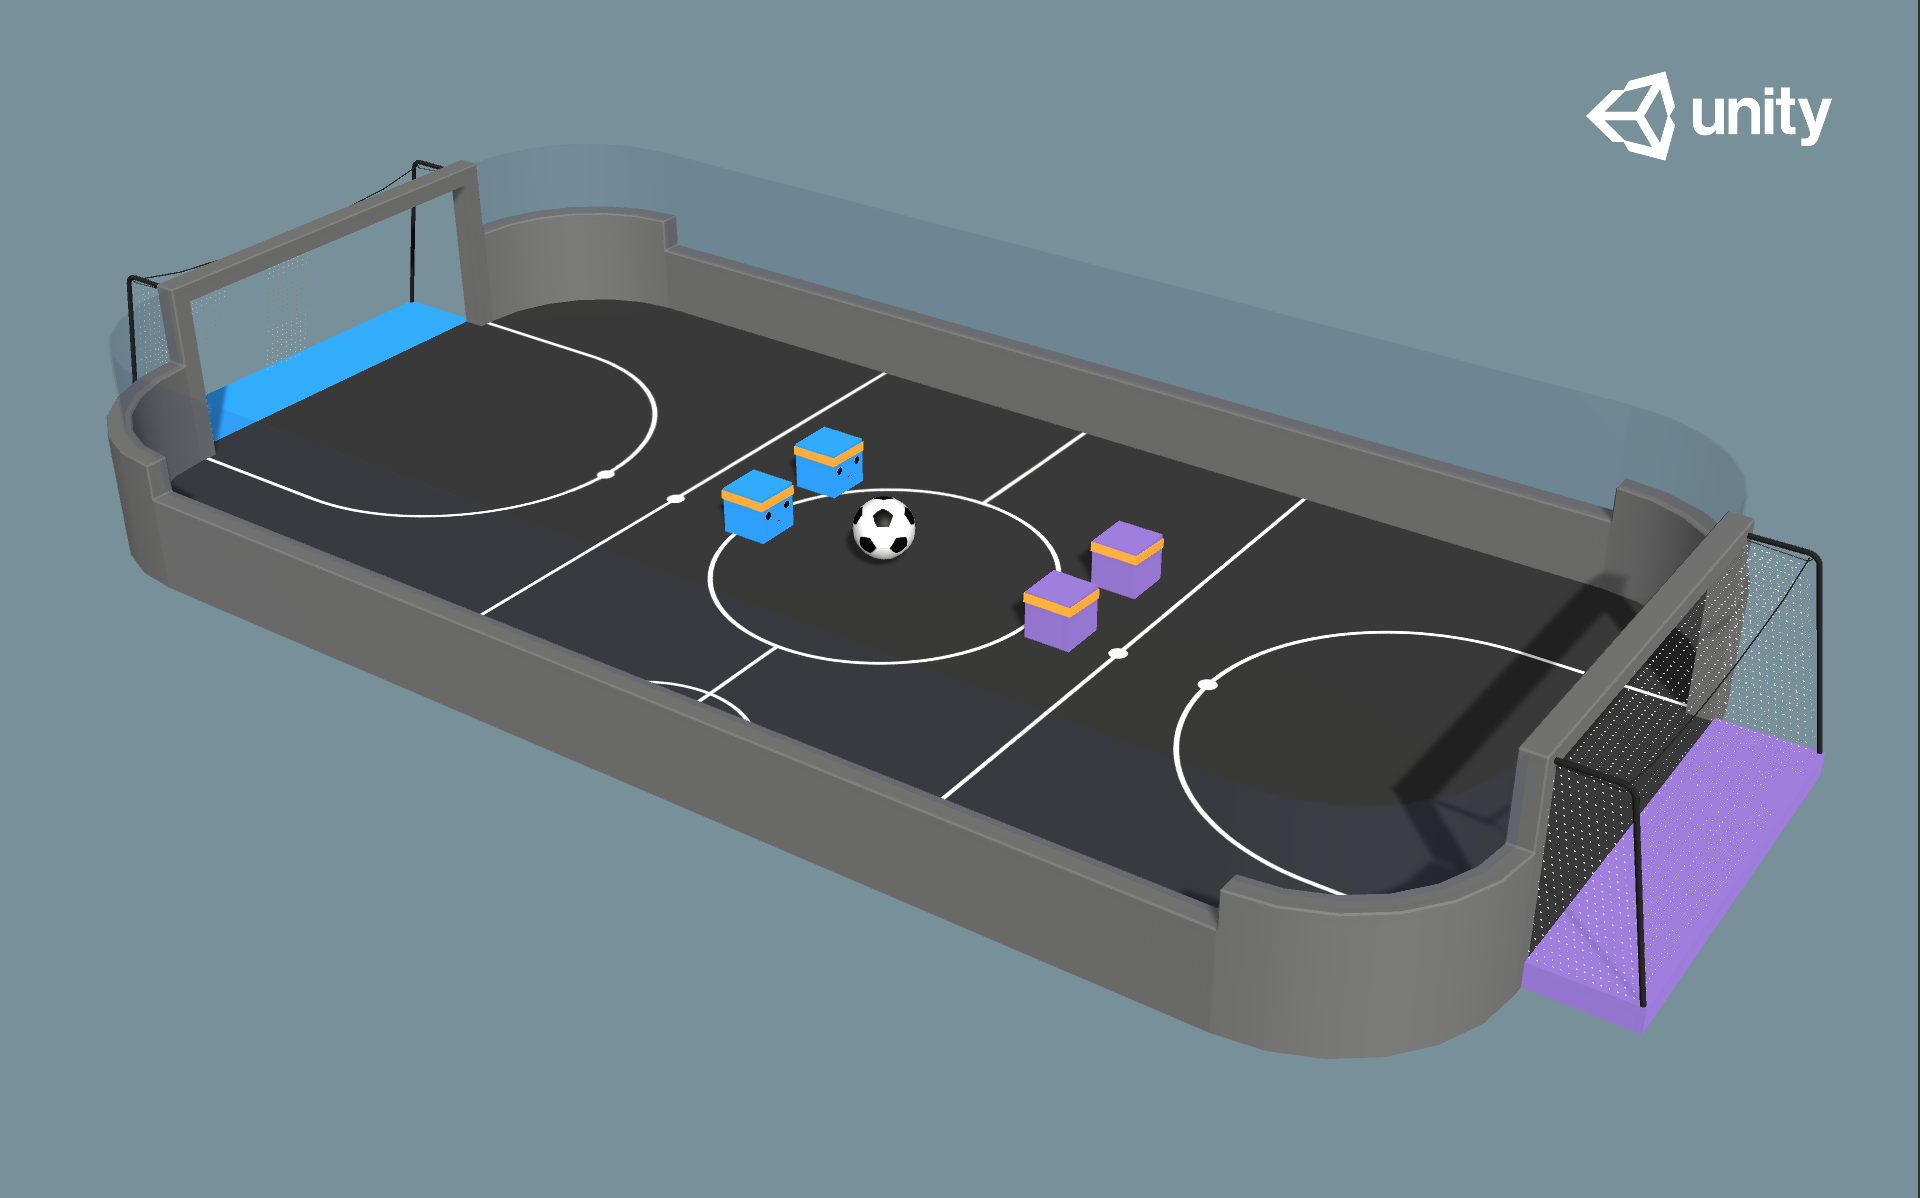
\includegraphics[width=\textwidth]{img/soccer_twos.png}
	\caption{Die visualisierte 3D-Spielumgebung von ``Soccer Twos'' des Unity \ac{ML}-Agents Toolkits. Die zwei Teams in Blau und Pink mit jeweils zwei blockförmigen Agenten stehen sich gegenüber, während der Fußball im Mittelkreis liegt. \cite{juliani2020}}
	\label{fig:soccer_twos_3d}
\end{figure}

Der Aktionsraum eines Agents ist diskret und umfasst die drei Dimensionen ``Vorgehen oder Zurückgehen'', ``Rechtsgehen oder Linksgehen'' sowie ``Linksdrehen oder Rechtsdrehen''. Für jede Dimension kann ein Wert aus \(\{0,1, 2\}\) gewählt werden, wobei \(0\) für keine Ansteuerung auf dieser Dimension steht, \(1\) für die zuerst genannte Aktion und \(2\) für die zweite. Zum einfachen Vorwärtsgehen sieht der Aktionsvektor somit wie folgt aus: \([1, 0, 0]\) oder schräg Vorwärts und Links: \([1, 2, 0]\). Es gibt somit 27 mögliche diskrete Aktionen.
Die Aktionen werden während eines Spiels für alle Agents gleichzeitig definiert und in einem 4-elementigen Dictionary übergeben.

Der Beobachtungsraum besteht aus einem Vektor mit 336 Dimensionen. Diese Dimensionen ergeben sich aus mehreren Strahlen (sogenannten Ray-Casts), die die Umgebung eines Agents abtasten. Konkret werden 11 Strahlen nach vorne ausgesendet, die einen Bereich von 120° abdecken, und 3 Strahlen nach hinten, die einen Bereich von 90° abdecken. Jeder dieser Strahlen kann 6 verschiedene Objekttypen erkennen und die Entfernung zu diesen Objekten messen. Um Bewegungsabfolgen zu erkennen, werden die Daten von drei aufeinanderfolgenden Beobachtungen zusammengeführt. %todo: klären wie die Dokumentation auf 336 kommt

Jedes Spiel wird entweder für 1000 Iterationen oder bis ein Tor erzielt wird gespielt. Die Belohnungsfunktion verleiht eine positive Belohnung von \(1 - \text{akkumulierte Zeitstrafe}\), wenn ein Tor erzielt wird. Zu Beginn einer Episode wird die Zeitstrafe auf \(0\) gesetzt und dann bei jedem Update um \( \frac{1}{\text{max Schritte}} \). Diese Berechnung der Belohnung trägt somit dazu bei, dass vor allem das schnelle Schießen eines Tores unterstützt wird.  Erhält ein Team ein Gegentor, wird eine negative Belohnung von \(-1\) verhängt, um so die Verteidigung des eigenen Tores anzureizen.
%todo: erweiterung beschreiben (lasse fragen)


\section{Multi Agent \acl{RL}}

Bei ``Soccer Twos'' handelt es sich um ein \ac{MARL}-Problem, welches ein Teilgebiet des normalen \ac{RL} darstellt. \ac{MARL} befasst sich mit Umgebungen, in denen mehrere Agenten agieren und somit auch miteinander interagieren können und sich durch ihre Aktionen gegenseitig beeinflussen.

Diese Umgebungen sind dezentral oder zentral aufgebaut. In einer dezentralen Umgebung wird jeder Agent alleine und unabhängig von den anderen Agenten trainiert, was bedeutet, dass jeder weiterhin seine eigene Belohnungsstruktur, Beobachtungen und Aktionen hat und im Lernprozess keine Informationen zwischen den Agenten geteilt werden. Dies hat den Vorteil, dass jeder Agent alleine trainiert werden kann und die anderen Agenten einfach als Teil der Umgebung wahrnimmt. Eine derartige Struktur hat jedoch den großen Nachteil, dass sie eine nicht-stationäre Umgebung erzeugt, auf die viele \ac{RL}-Algorithmen angewiesen sind.
In einer zentralen Umgebung hingegen gibt es eine übergeordnete Struktur, welche die Beobachtungen und Belohnungen aller Agenten sammelt und verarbeitet. Dadurch kann eine einzige gemeinsame Policy erlernt werden und das Wissen wird zwischen den Agenten geteilt. \cite{Tan:1993} %https://web.media.mit.edu/~cynthiab/Readings/tan-MAS-reinfLearn.pdf
%Zentral und dezentral https://huggingface.co/learn/deep-rl-course/en/unit7/multi-agent-setting

Neben der Art der Umgebung lässt sich weiter zwischen zwei Interaktionstypen der Agenten unterscheiden \cite{10.1007/11691839_1}. In kooperativen Umgebungen agieren mehrere Agenten, um eine gemeinsame Belohnung zu maximieren. Es ist also das Ziel, dass die Agenten zusammen eine Aufgabe lösen und sich gegenseitig unterstützen. In konfrontativen Umgebungen treten mehrere Agenten gegeneinander an und versuchen, ihre eigene Belohnung zu maximieren, während die Belohnung des Gegners minimiert wird.
Weiter ist es möglich, dass diese beiden Arten auch in gemischter Form auftreten und es somit in einer Umgebung sowohl kooperative Agenten gibt, die aber konfrontativ gegenüber anderen auftreten. Genau um eine solche gemischte Umgebungsform handelt es sich auch bei dem ``Soccer Twos''-Problem. Zwei Agenten eines Teams spielen gemeinsam kooperativ gegen ein anderes Team, welches einen konfrontativen Gegner darstellt.


%ggf. noch so sagen das meisten rl probleme in der vergangenheit nur einen agent betrachtet haben aber marl für realität etc. viel interessanter ist und daher in der vergangeheit jetzt mehr erforscht wurde aber eben auch komplexer ist.

